\documentclass[report]{jsbook}
\usepackage{amsthm,amsmath,amssymb,listings,ascmac,jlisting,docmute,bm}
\usepackage[dvipdfmx]{graphicx}
% \usepackage[dviout]{graphicx}

\lstset{%
  language={C},
  basicstyle={\small},%
  identifierstyle={\small},%
  commentstyle={\small\itshape},%
  keywordstyle={\small\bfseries},%
  ndkeywordstyle={\small},%
  stringstyle={\small\ttfamily},
  frame={tb},
  breaklines=true,
  columns=[l]{fullflexible},%
  % numbers=left,%
  xrightmargin=0zw,%
  xleftmargin=3zw,%
  numberstyle={\scriptsize},%
  stepnumber=1,
  numbersep=1zw,%
  lineskip=-0.5ex%
}

\makeatletter
\long\def\@makecaption#1#2{{\small
  \advance\leftskip .0628\linewidth
  \advance\rightskip .0628\linewidth
  \vskip\abovecaptionskip
  \sbox\@tempboxa{#1\hskip1zw\relax #2}%
  \ifdim \wd\@tempboxa <\hsize \centering \fi
%  #1\hskip1zw\relax #2\par
  #1{\hskip1zw\relax}#2\par
  \vskip\belowcaptionskip}}
\makeatother


\title{近似的メッセージ伝播法に基づくパイロット汚染の軽減}
\author{豊橋技術科学大学電気・電子情報工学課程\\藤塚 拓実\\\\指導教員 竹内啓悟\\} 
\date{\today}

\begin{document}
\maketitle
\chapter{概要}
今日,2020年までに,第5世代移動通信システム(5G)の国内での実用化に向けて,各研究機関,企業,大学が様々な研究・実験を実施している.

5Gの中心的技術として,大規模MIMOがある.大規模MIMOとは,基地局のアンテナを大量に保有することで,無線通信のスループットの向上を図る通信技術である.

しかし,信号を復調する際,従来の計算方法では,アンテナ数の増加に伴い,爆発に計算量が増えてしまう.そこで,本研究では,大規模MIMOの実現に向けて,復調の新たな計算方法として,人工知能の分野で提案された,近似的メッセージ伝播法(AMP)を用いてシミュレーションを行った.
\chapter*{謝辞}
本研究を進めるにあたり,お忙しい中,終始熱心なご指導をいただいた竹内啓悟先生に深謝いたします.また,竹内研究室の皆様には日頃から数々の助言をいただきました.ここに,協力していただいた皆様へ心から感謝の気持ちと御礼を申し上げたく,謝辞にかえさせていただきます.  
% 目次の表示
\tableofcontents
\newpage
\chapter{はじめに}
\section{研究背景}
2020年東京オリンピック・パラリンピック大会に向けて,日本国内の情報通信基盤(ICT)を飛躍的に向上させる戦略が,総務省を中心として活発になっている.その戦略の一つとして,第5世代移動通信システム(以下「5G」)の実現がある\cite{soumu_suzuki}.

近年スマートフォンのような高機能端末が一般層へ広く普及したことを起爆剤として,M2M(Machine to Machine)やIoT(Internet of Things)が拡大していくことが予想されている.そのため,現行の4G/LTEよりもさらに,超高速・大容量のモバイル通信ネットワークとして,5Gの実現が求められる\cite{suyama}.

\section{大規模MIMO(Massive MIMO)}
5Gの中心的役割を担う技術が,大規模MIMO(massive MIMO)である.MIMO( Multiple Input Multiple Output)とは,送受信側が複数のアンテナを持ち合わせ持つことにより,データレート増加,ダイバーシチによる特性改善を図ることができるものである\cite{goldsmith}.4G/LTEで既に使用されているMIMOでは,通信基地局のアンテナは2,4,8本程度しか持ち合わせていないが,大規模MIMOは,同一の基地局を利用するユーザ数十人を,100以上の受信アンテナでカバーすることで多入力,多出力のシステムを実現する\cite{emil}\cite{Vidit}.図\ref{fig:mimo}に概念図を示す.
\begin{figure}[htbp]
  \begin{center}
    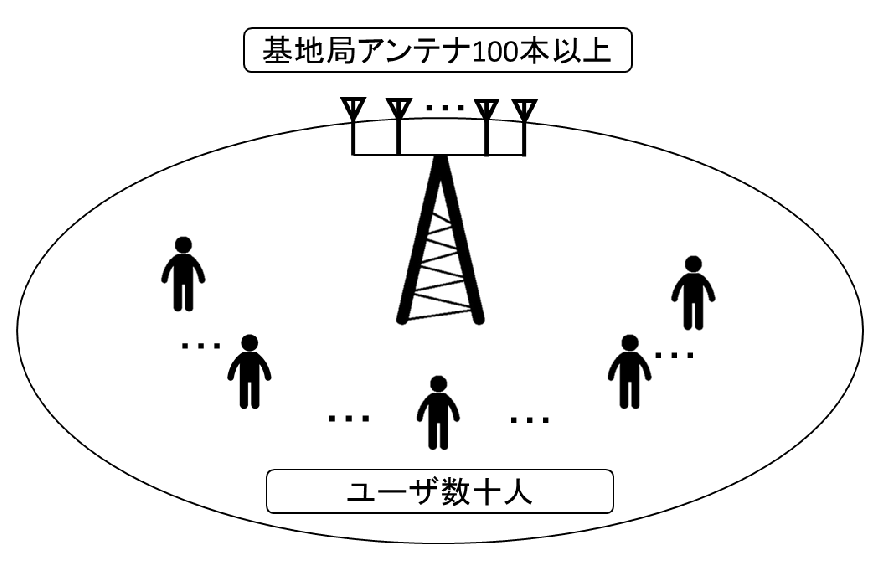
\includegraphics[clip,width=10.0cm]{./mimo.eps}
    \caption{大規模MIMOの概念図}
    \label{fig:mimo}
  \end{center}
\end{figure}

大規模MIMOでは,ユーザと受信側がともに複数のアンテナを持ち合わせるポイント・ツー・ポイント(point-to-point)MIMOではなく,単一のアンテナを持つ複数人のユーザが多数のアンテナを持つ受信機にアクセスするマルチユーザMIMOを想定する.なぜならば,ユーザが複数アンテナを保持すると,端末が高価になり,かつ端末の中の距離が近いアンテナ同士が干渉を起こし,重複による利得が減衰する可能性があるためである\cite{Marzetta}.

大規模MIMOの時分割複信(TDD)システムでは,アップリンク(ユーザから基地局への通信)で得られた通信路状態情報(CSI)をもとに,ダウンリンク(基地局からユーザへの通信)では,プリコーディングを行うことで,ダウンリンクの通信を容易にする.よって,アップリンクのCSI推定が非常に重要な処理となる\cite{Khansefid}.CSIを推定する際,アンテナ数を無限大に考えた場合,無相関のノイズや高速フェージングの影響は無視できるが,パイロット汚染(Pilot Contamination)\cite{Marzetta}と呼ばれる問題が現象が発生する.

\section{パイロット汚染(Pilot Contamination)}
\label{sec:pilot_contamination}
データを送信する際,ユーザはパイロット信号と呼ばれる基地局側にも既知のデータを送ることで,基地局側はCSIを推定するが,隣接する基地局同士(ユーザ同士でも)が同じパイロットを送信してしまうと,基地局が通信路を学習する過程で,誤って別の基地局の通信路を学習してしまう現象がパイロット汚染である.パイロット信号を送信する時間が短いと,パイロット信号が等しくなる可能性が高くなるため,パイロット汚染が発生しやすい.つまり,パイロット信号に必要な時間は基地局のアンテナ数には依存せず,ユーザの数に依存して増大してしまう.このパイロット汚染が基地局間干渉として,大規模MIMOの通信には発生する.

この基地局間干渉(パイロット汚染)を抑制する方法として,基地局ごとにでパイロットの送信を時間シフトさせて送信する\cite{Appaiah}方法がある(図\ref{fig:shiftedframe}を参照).隣接する基地局は,お互いのユーザの信号を受け取ってしまうが,パイロット信号を送信する時間をずらすことで,パイロット汚染を防ぎ,基地局間干渉を抑制することができる.本研究では,パイロット信号を時間シフトさせてシミュレーションを行った.

\begin{figure}[htbp]
  \begin{center}
    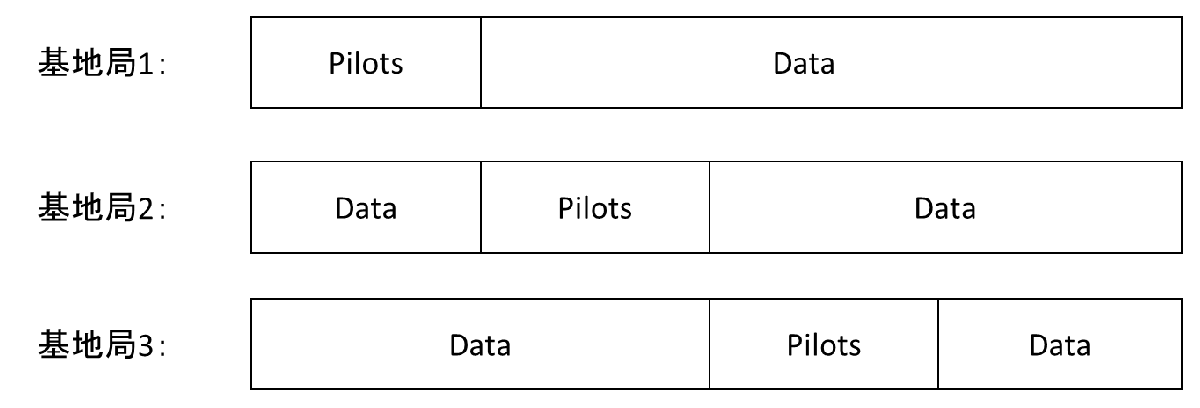
\includegraphics[clip,width=10.0cm]{./shiftedframe.eps}
    \caption{パイロット行列を時間シフトしたデータ構造  出典:\cite{Appaiah}Fig.1を修正}
    \label{fig:shiftedframe}
  \end{center}
\end{figure}


\section{研究目的}
本研究では,大規模MIMO通信におけるアップリンクにおいて,基地局側が通信路と送信データを同時に推定するシミュレーションを行う.その際,\ref{sec:pilot_contamination}にて説明した基地局間干渉を考慮したうえで,基地局側が信号を復調する際,別の基地局の信号と自身の基地局の信号を分離できるように,基地局ごとにでパイロットの送信を時間シフトさせて送信することで,パイロット汚染を抑制することを目的とする.

\section{研究内容}
ユーザが送った信号は通信路を通って基地局のアンテナへ送られる.このとき,基地局で受け取る受信信号行列を$\bm{Y}$,通信路行列を$\bm{H}$,送信データ行列を$\bm{X}$,AWGN通信路を仮定し,ノイズを$\bm{W}$とすると以下のような式で表せる.
\begin{equation}
  \label{eq:mimosystem}
  \bm{Y} = \bm{H}\bm{X}+\bm{W}
\end{equation}
このとき,基地局側からみて,$\bm{H}$と$\bm{X}$は未知であり,基地局は$\bm{Y}$より$\bm{H}$と$\bm{X}$を推定しなければならない.

本研究では,大規模MIMOの復調の計算方法として,近似的メッセージ伝播法(Approximate Message Passing 以下「AMP」)を用いる.AMPは,人口知能分野で提案された確率伝播法(Belief Propagation BP)を基礎として発展した統計学的手法であり.もともとは,圧縮センシングの分野で提案された手法である\cite{Donoho}.

AMPアルゴリズムを用いて,二つの行列の積の情報より,元の二つの行列を推定する体系的な理論は,参考文献\cite{kabashima}の著者である樺島祥介氏らによって考案された.参考文献\cite{kabashima}では,行列分解のためのAMPアルゴリズムの導出と理論的な数値特性の評価を行っている.本研究では,AMPアルゴリズムを使い,大規模MIMOシステムで通信路とデータを推定する数値シミュレーションを行った.具体的には,式(\ref{eq:mimosystem})に示すように,推定する二つの行列を通信路$\bm{H}$と送信データ$\bm{X}$として,送信データにはパイロット信号を付加する.さらに,二つの行列の積の結果に白色雑音$\bm{W}$とを足したものを大規模MIMOのアンテナが受け取る受信信号$\bm{Y}$として,受信信号より通信路と送信データを推定する.

\chapter{提案手法}
\section{アップリンクマルチユーザMIMO}
本研究は,複数ユーザが基地局に情報を送るアップリンクを想定して研究を行った.ユーザ数を$K$,受信アンテナ数を$N$とし,ユーザは単一の送信アンテナを持つことを想定する.また,簡単のため,フェージング係数が観測時間$T$の間一定であるブロックフェージング通信路を仮定する.受信信号$\boldsymbol{Y}\in\mathbb{C}^{N\times T}$は式(\ref{eq:ReceiveSignal})にて与えられる.
\begin{equation} 
	\label{eq:ReceiveSignal}
	\boldsymbol{Y} = \frac{1}{\sqrt{N}}\boldsymbol{HX+W}.
\end{equation}
$1/\sqrt{N}$は正規化定数であり,アンテナ数の上昇による電力の上昇を抑える.$\boldsymbol{X}\in\mathbb{C}^{K\times T}$は全ユーザの送信信号であり,$\boldsymbol{H}\in\mathbb{C}^{N\times K}$はすべてのユーザとアンテナ間のフェージング係数である.ここで,$\boldsymbol{H}$に関して,すべての行列成分は,互いに独立で同一の分布(independent and identically distribution : i.i.d)のレイリーフェージングに従うと仮定する.具体的には,それぞれが独立した円対称複素ガウス雑音(circularly symmetric complex Gaussian : CSCG)であり,分散は1とした.また,$\boldsymbol{W}\in\mathbb{C}^{N\times T}$は受信時に生じる雑音のことであり,それぞれが独立した円対称複素ガウス雑音で,分散は定数$N_0$とした.

ここで,基地局間干渉のため,ユーザーを二つのグループに分ける.一方のグループは自分の基地局のエリアに存在するユーザで,$K/2$人で構成され,残る$K/2$人のユーザは別の基地局のエリアのユーザであり,自分の基地局の信号に干渉してくる.これを踏まえ,$\boldsymbol{X}$を式(\ref{eq:SendSignal})のように定義する.
\begin{equation} 
	\label{eq:SendSignal}
	\boldsymbol{X} =  \left(
		\begin{array}{cccc}
			\boldsymbol{X}_{11} &\boldsymbol{X}_{12} &\boldsymbol{P}\\
			\boldsymbol{P} &\boldsymbol{X}_{21} &\boldsymbol{X}_{22}.
		\end{array}
	\right)
\end{equation}
$\boldsymbol{P}$は$K/2\times T_{p}$のパイロット行列であり,基地局側にとってこの信号は既知である.$\boldsymbol{X}$の行方向は観測時間$T$であるので,$\boldsymbol{P}$の送信時間の違いによって,行列(\ref{eq:SendSignal})は上半分と下半分で基地局を分けている.また,$\boldsymbol{X}$信号はそれぞれ,式(\ref{eq:QPSK})のような電力1のQPSK信号である.電力1というのは,ユーザの長期的な平均電力とする.
\begin{equation} 
	\label{eq:QPSK}
	x_{kt} = \{u+jv:u,v=\pm\sqrt{1/2}\}.
\end{equation}

\section{通信路推定とデータ推定}
受信側で推定するデータを$\hat{\boldsymbol{X}}$として,ここでは,推定するデータは事後平均推定
\begin{equation} 
	\label{eq:PosterorMean}
	\hat{\boldsymbol{X}}=\mathbb{E}[\boldsymbol{X}|\boldsymbol{Y},\boldsymbol{P}]
\end{equation}	
を目標とする.しかし,大規模MIMOシステムでは,式(\ref{eq:PosterorMean})は$K,N,T$の上昇に伴い,指数関数的に上昇するため現実的な時間で解くことは,不可能である.そこで,AMPアルゴリズムを用いる.詳しい式の導出は,\ref{sec:AMP}章に譲る.AMPアルゴリズムを使う条件として,$N,K,T,Tp$が無限大に近く,$\alpha=K/N$,$\beta=T/N$,$\tau=T_{p}/T$が一定で保たれる必要がある.AMPアルゴリズムでは,表\ref{tb:Message}で示される8つのメッセージをそれぞれ交換することで推定を行っていく.初期値として,パイロット信号が入っている$(k,t) \in \{1,...,K/2\}\times \{T-T_{p}+1,...,T\}$もしくは$(k,t) \in \{K/2+1,...,K\}\times \{1,...,T_{P}\}$のとき,$\hat{x}_{kt}=x_{kt}$,$\xi_{kt}=0$となり,パイロット信号が入っていない,それ以外の成分は$\hat{x}_{kt}=0$,$\xi_{kt}=1$とした.また,他の要素は,$\hat{h}_{nk}=0$,$\eta_{nt}=1$,$\overline{I}_{nt}=0$,$\zeta_{nt}=0$とした.
\begin{table}[htb]
	\begin{center}
		\caption{AMPアルゴリズムで使用されるメッセージ \label{tb:Message}}
		\begin{tabular}{|c|c|} \hline
			$\hat{x}_{kt}$ & $x_{kt}$の事後平均 \\ \hline
			$\xi_{kt}$ & $x_{kt}$の事後分散 \\ \hline
			$\overline{x}_{kt}$ & $x_{kt}$の外部平均 \\ \hline
			$\overline{\xi}_{kt}$ & $x_{kt}$の外部分散 \\ \hline\hline
			$\hat{h}_{nk}$ & $h_{nk}$の事後平均 \\ \hline
			$\eta_{nk}$ & $h_{nk}$の事後分散 \\ \hline\hline
			$\overline{I}_{nt}$ & $y_{nt}$の干渉の平均 \\ \hline
			$\zeta_{nt}$ & $y_{nt}$の干渉の分散 \\ \hline
		\end{tabular}
	\end{center}
\end{table}

ここで,各メッセージを計算するための定義式を記す.まず,干渉を差し引いた出力$z\in\mathbb{C}$は
\begin{equation} 
	\label{eq:z}
	z_{nt}=\frac{y_{nt}-\overline{I}_{nt}}{N_{0}+\zeta_{nt}}
\end{equation}
と定義する.$\Re[x_{kt}]$の軟判定関数として,以下のような関数を定義する.
\begin{equation} 
	\label{eq:fk}
	f_{k}(u;v)=\frac{1}{\sqrt{2}}
			\frac{e^{\sqrt{2}u/v}-e^{-\sqrt{2}u/v}}{e^{\sqrt{2}u/v}+e^{-\sqrt{2}u/v}}.
\end{equation}
複素関数$A_{kt}(z)$として,以下のような関数を定義する.
\begin{equation} 
	\label{eq:Akt}
	A_{kt}(z)=\Re[z]\frac{\partial f_{k}}{\partial u}(\Re[\overline{x}_{kt}];\overline{\xi}_{kt})+j\Im[z]\frac{\partial f_{k}}{\partial u}(\Im[\overline{x}_{kt}];\overline{\xi}_{kt}).
\end{equation}
データ推定に関わるメッセージの式を以下に示す.
\begin{equation} 
	\label{eq:x_h}
	\hat{x}_{kt}=f_{k}(\Re[\overline{x}_{kt}],\overline{\xi}_{kt})+jf_{k}(\Im[\overline{x}_{kt}],\overline{\xi}_{kt}),
\end{equation}
\begin{equation} 
	\label{eq:xi}
	\xi_{kt} = 1 - |\hat{x}_{kt}|^2,
\end{equation}
\begin{equation} 
	\label{eq:x_b}
	\overline{x}_{kt} = 
		\frac{\overline{\xi}_{kt}}{\sqrt{N}}
			\sum_{n=1}^{N}\hat{h}^{*}_{nk}z_{nt}
			+\left(
				1-\frac{\overline{\xi}_{kt}}{N}\sum_{n=1}^{N}\eta_{nk}|z_{nt}|^2
			\right)
			\hat{x}_{kt},
\end{equation}
\begin{equation} 
	\label{eq:xi_b}
	\overline{\xi}_{kt}=
	\left(
		\frac{1}{N}
		\sum_{n=1}^{N}
			\frac
			{|\hat{h}_{nk}|^{2}}
			{N_{0}+\zeta_{nt}}
	\right)^{-1}.
\end{equation}
通信路推定に関するメッセージの式を示す.
\begin{equation}
	\label{eq:h_h}
	\hat{h}_{nk}=
	\frac
		{\eta_{nk}}
		{\sqrt{N}}
	\sum_{t=1}^{T}
		\hat{x}^{*}_{kt}z_{nt}
	+
	\left(
		1-\eta_{nk}
	\right)
	\hat{h}_{nk}
	-
	\frac
		{\eta_{nk}}
		{N}
	\sum_{t=1}^{T}
		\overline{\xi}_{kt}
		A^{*}_{kt}
		\left(
			\hat{h}_{nk}^{*}
			z_{nt}
		\right)
		z_{nt},	
\end{equation}
\begin{equation}
	\label{eq:eta}
	\eta_{nk}=
	\left(
		1+
		\frac{1}{N}
		\sum^{T}_{t=1}
			\frac
			{|\hat{x}_{kt}|^{2}}
			{N_{0}+\zeta_{nt}}
	\right)^{-1}.
\end{equation}
最後に,干渉に関するメッセージの式を示す.
\begin{equation}
	\label{eq:I_b}
	\overline{I}_{nt}=
		\frac{1}{\sqrt{N}}
		\sum_{k=1}^{K}
			\hat{h}_{nk}\hat{x}_{kt}
		-
		\frac{1}{N}
		\sum^{K}_{k=1}
			\overline{\xi}_{kt}
			A_{kt}
			\left(
				\hat{h}_{nk}^{*}
				z_{nt}
			\right)
			\hat{h}_{nk}
		-
		\frac{1}{N}
		\sum^{K}_{k=1}
			\eta_{nk}
			|\hat{x}_{kt}|^{2}
			z_{nt},
\end{equation}
\begin{equation}
	\label{eq:zeta}
	\zeta_{nt}=
		\sum_{k=1}^{K}
			\left(
				\eta_{nk}\xi_{kt}
				+
				\eta_{nk}|\hat{x}_{kt}|^{2}
				+
				|\hat{h}_{nk}|^{2}\xi_{kt}
			\right)
\end{equation}
AMPアルゴリズムでは,式(\ref{eq:x_h})-(\ref{eq:zeta})を計算することで,通信路とデータを同時推定する.
\section{メッセージの初期化と更新順序}
ここで,上記メッセージの初期化と更新順序について明記しておく.初期値について表\ref{tb:init_Message}に示す.
\begin{table}[htb]
	\begin{center}
		\caption{メッセージの初期値\label{tb:init_Message}}
		\begin{tabular}{|c|c|} \hline
			$\hat{x}_{kt}$ & pilot信号・・・$x$と同値,その他・・・0 \\ \hline
			$\xi_{kt}$ & pilot信号・・・0 その他・・・1 \\ \hline
			$\overline{x}_{kt}$ & pilot信号・・・$x$と同値,その他・・・0 \\ \hline
			$\overline{\xi}_{kt}$ & 1 \\ \hline\hline
			$\hat{h}_{nk}$ & 0\\ \hline
			$\eta_{nk}$ & 1\\ \hline\hline
			$\overline{I}_{nt}$ & 0\\ \hline
			$\zeta_{nt}$ & 0\\ \hline
		\end{tabular}
	\end{center}
\end{table}

計算順序について,図(\ref{fig:flow_message})にフローチャートを示す.
\begin{figure}[htbp]
  \begin{center}
    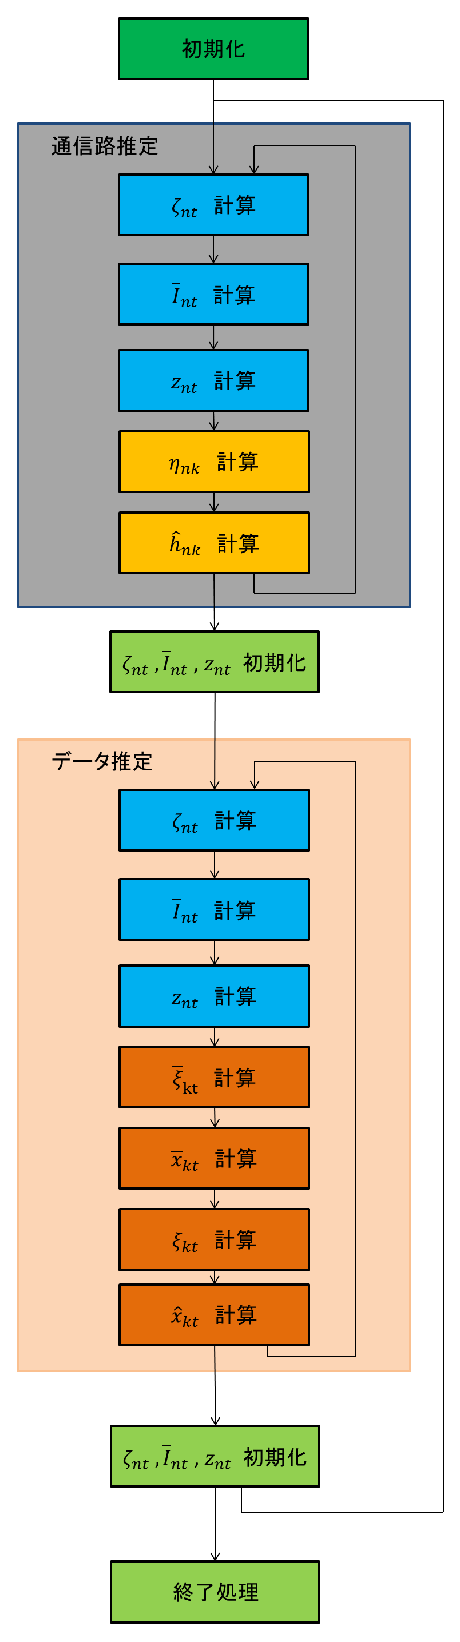
\includegraphics[clip,width=5.0cm]{./flow_message.eps}
    \caption{メッセージの計算順序}
    \label{fig:flow_message}
  \end{center}
\end{figure}
\chapter{導出}
\section{近似的確率伝搬法 (Belief Propagetion BP)}
\section{近似的メッセージ伝播法 (Approximate Message Passing AMP)}

\newpage
\chapter{シミュレーション結果}
\section{シミュレーション条件}
\label{sec:contdition}
シミュレーション条件として,基地局数2,基地局のアンテナ数128本,基地局当たりのユーザ数16人,送信フレーム長1000,パイロット信号の長さ300,通信路/データ推定器内における反復回数30回,両者の間の反復回数3回の場合を想定した.送信するデータは電力1のQPSK信号であり,送信するデータ構造は図\ref{fig:data_structure}に示す.
\begin{figure}[htbp]
  \begin{center}
    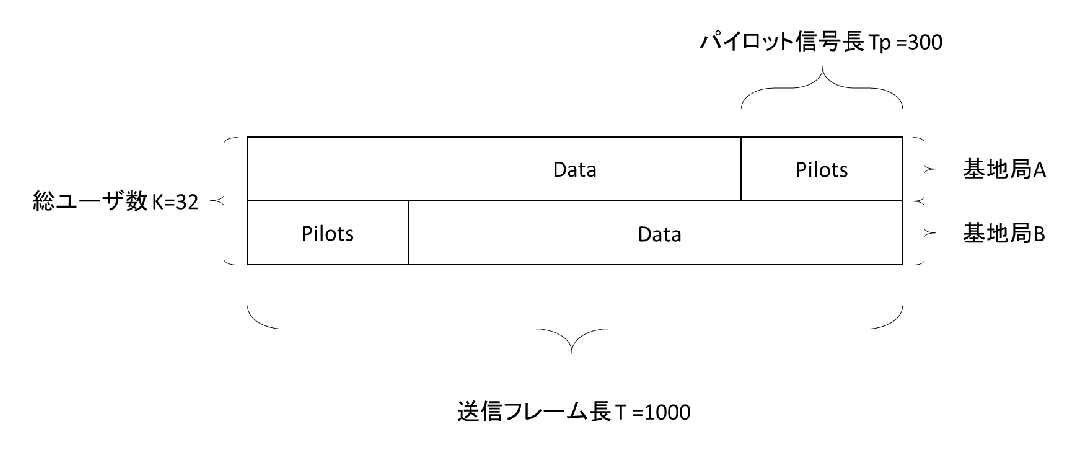
\includegraphics[clip,width=10.0cm]{./data_structure.eps}
    \caption{送信されるデータ構造}
    \label{fig:data_structure}
  \end{center}
\end{figure}

また,計算順序は以下のとおりである.
\begin{enumerate}
	\item 初期処理(通信路とデータの生成,メッセージの初期化)
	\item 通信路推定を30回繰り返す \label{estimate_h}
	\item データ推定を30回繰り返す  \label{estimate_x}
	\item \ref{estimate_h}.\ref{estimate_x}.を3回繰り返す
	\item 終了処理
\end{enumerate}
なお,以下に示す結果はすべて50回のアンサンブル平均で示す.
\section{通信路推定}
横軸に反復回数,縦軸に通信路推定の平均二乗誤差(MSE)をとり,SNRごとに出力したものを図\ref{fig:mse_h}に示す.反復回数30回ごとにデータ推定を行い,再び通信路推定を行ったときにMSEが減少していることが確認できる.また,SNR=10dBのときの時間シフト送信データフレームと,同期送信データフレームのMSEの比較した図を図\ref{fig:mse_h_comparison}に示す.一回目の通信路推定では,シフトフレームはMSE=0.126566に対し,同期フレームはMSE=0.095458であったが最終的にシフトフレームはMSE=0.025941,同期フレームはMSE=0.026116であり,反復を振り返すと,二つのMSEの差は小さくなった.
\begin{figure}[htbp]
  \begin{center}
    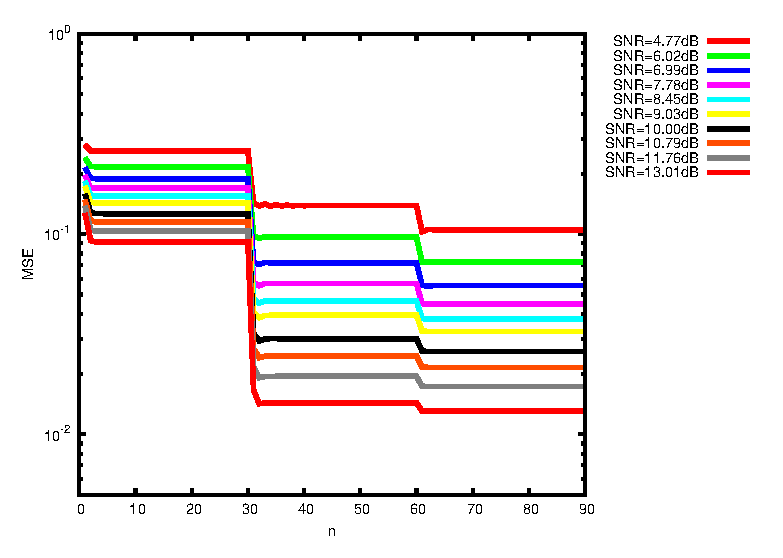
\includegraphics[clip,width=10.0cm]{./mse_h.eps}
    \caption{通信路推定の平均二乗誤差}
    \label{fig:mse_h}
  \end{center}
\end{figure}

\begin{figure}[htbp]
  \begin{center}
    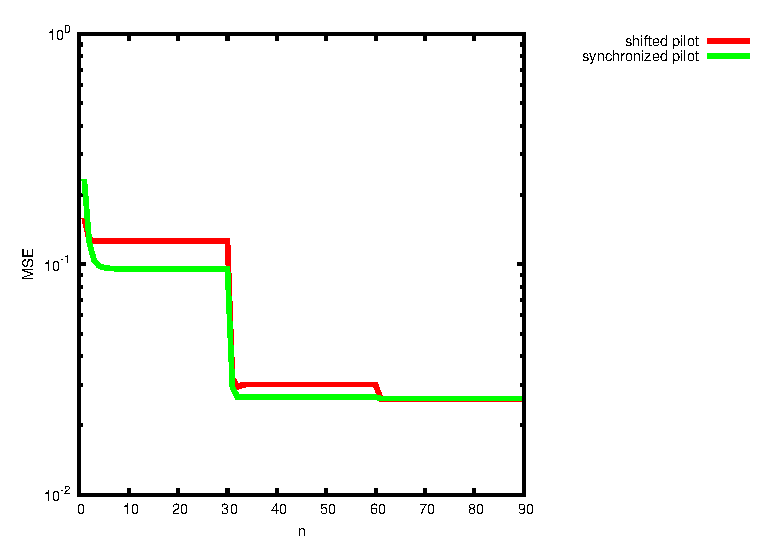
\includegraphics[clip,width=10.0cm]{./mse_h_comparison.eps}
    \caption{通信路推定の平均二乗誤差 時間シフトフレームと同期フレームの比較(SNR=10dB)}
    \label{fig:mse_h_comparison}
  \end{center}
\end{figure}
\section{データ推定}
横軸に反復回数,縦軸にデータ推定のビット誤り率をとり,SNRごとに出力したものを図\ref{fig:bit_err}に示す.反復回数30回ごとに通信路推定を行い,再びデータ推定を行ったときにBERが減少していることが確認できる.また,SNR=10dBのときの時間シフト送信データフレームと,同期送信データフレームのBERを比較した図を図\ref{fig:bit_err_comparison}に示す.一回目のデータ推定では,シフトフレームBER=0.011804に対し,同期フレームはBER=0.002713であったが最終的にシフトフレームはBER=0.001163,同期フレームはBER=0.001170であり,反復を振り返すと,二つのBERの差は小さくなった.
また,横軸にSNR,縦軸にデータ推定のビット誤り率をとり出力したものを図\ref{fig:sn_bit_err}に示す.SNRの上昇に伴いBERも減少していくことが確認できた.
\begin{figure}[htbp]
  \begin{center}
    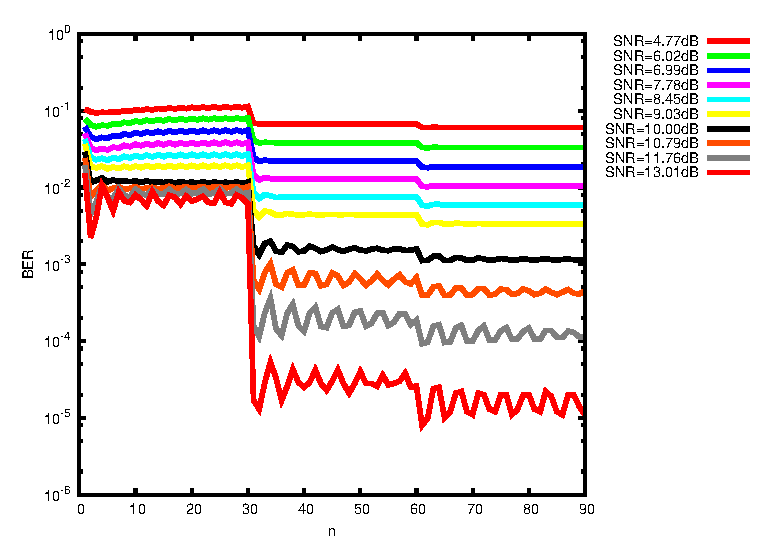
\includegraphics[clip,width=10.0cm]{./bit_err.eps}
    \caption{データ推定のBER}
    \label{fig:bit_err}
  \end{center}
\end{figure}
\begin{figure}[htbp]
  \begin{center}
    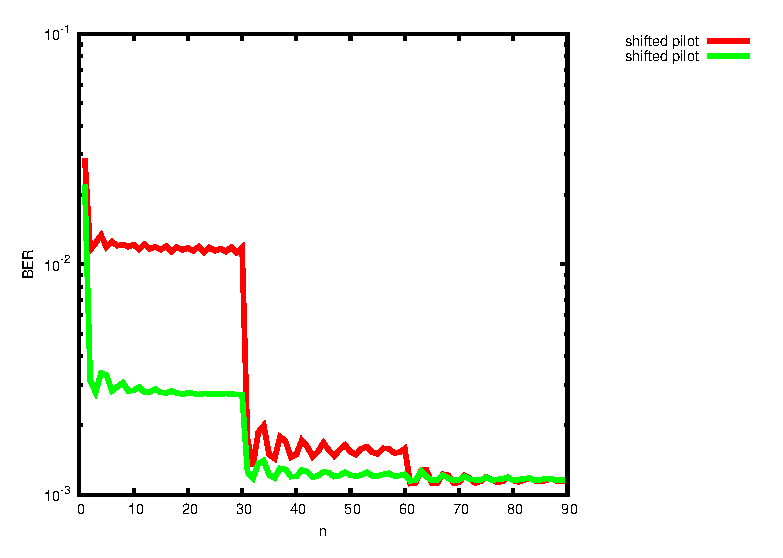
\includegraphics[clip,width=10.0cm]{bit_err_comparison.eps}
    \caption{データ推定のBER 時間シフトフレームと同期フレームの比較(SNR=10dB)}
    \label{fig:bit_err_comparison}
  \end{center}
\end{figure}
\begin{figure}[htbp]
  \begin{center}
    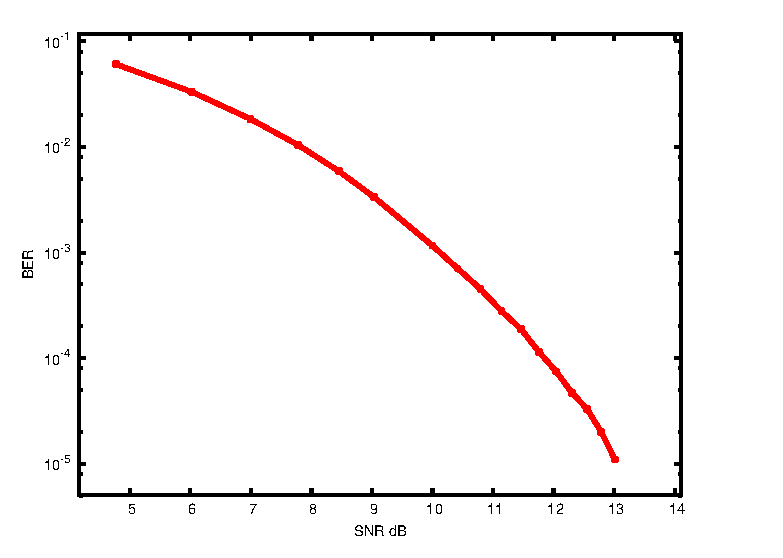
\includegraphics[clip,width=10.0cm]{./sn_bit_err.eps}
    \caption{データ推定のBER}
    \label{fig:sn_bit_err}
  \end{center}
\end{figure}
\newpage
\chapter{結論}
まず,通信路推定に関して説明する.パイロット汚染を抑制するために,式(\ref{eq:SendSignal})のようにパイロット信号を離して送信したが,パイロット汚染が発生しない場合,式(\ref{eq:SendSignal_all})のように基地局ごとにパイロット信号を時間的に並べて送信した方が通信路推定の精度は高い.
\begin{equation} 
	\label{eq:SendSignal_all}
	\boldsymbol{X} =  \left(
		\begin{array}{cc}
			\boldsymbol{P}_{1} &\boldsymbol{X}_{12}\\
			\boldsymbol{P}_{2} &\boldsymbol{X}_{21}.
		\end{array}
	\right)
\end{equation}
なぜならば,ユーザ同士の干渉は式(\ref{eq:I_b})が示すように,全ユーザの$\hat{x}_{kt}$がないと計算できないためである.しかし,データ推定した値を利用し,再び通信路推定を行うことで,時間シフトさせた送信データでも通信路推定を行うことができた.

次にデータ推定の結果について説明する.図(\ref{fig:bit_err})のように振動が発生している.原因として,近似的メッセージ伝搬法では,$N,K,T\to \infty$を仮定して計算式を導出しているため,有限の条件では必ず収束するとは限らないためだと考えられる\cite{kabashima}.

また,\ref{sec:contdition}と同様の条件で$\tau=0.3$の比率はそのままで,$T,Tp$を小さくした場合,推定値は発散してしまった.この原因も有限サイズのシステムによって推定精度が悪化したためだと考察される.

今後の課題として,$T,Tp$を小さくしても,推定値が発散せずに推定できるような計算式やアルゴリズムを改良することや,基地局数を増やしてシミュレーションを行うことが必要である.

\begin{thebibliography}{10}
  \bibitem{soumu_suzuki}
  鈴木 茂樹, ``2020年代に向けた情報通信政策の在り方-世界最高レベルの情報通信基盤の更なる普及・発展に向けて-,''{\sl 総務省}, \\ {https://www.nic.ad.jp/ja/materials/iw/2014/proceedings/d2/d2-suzuki.pdf}, Oct. 2014.
  \bibitem{suyama}
  須山 聡, シン キユン, 小原 辰徳, 角 誠, 中島 光雅, 奥村 幸彦, ``高周波数帯を用いた超高速MassiveMIMO伝送の基本特性,'' {\sl 信学技報}, Mar. 2014.
  \bibitem{goldsmith}
  A. Goldsmith, ``Wireless Communication,'' {\sl Cambridge University Press}, 2005, (訳) 小林 岳彦, 岩切 直彦, 大坐畠 智, 幸谷 智, 高橋 賢, 森 香津夫, 山嵜 彰一郎, ``ゴールドスミス ワイヤレス通信工学 基礎理論からMIMO,OFDM,アドホックネットワークまで,'' 丸善株式会社, p.297, 2007.
  \bibitem{emil}
  E. Bj${\rm \ddot o}$rnspn, E. G. Larsson, M. Debbah,"Massive MIMO for Maximal Spectral Efficiency: How Many Users and Pilots Should Be Allocated?," {\sl IEEE trans. Wireless Commun.}, Oct. 2015.
  \bibitem{Vidit}
  V. Saxena, ``Pilot Contamination and Mitigation Techniques in Massive MIMO Systems,''{\sl Department of Electrical and Information Technology LTH, Sweden}, Oct. 2014.
  \bibitem{Marzetta}
  T. L. Marzetta, ``Noncooperative Cellular Wireless with Unlimited Numbers of Base Station Antennas,'' {\sl IEEE trans. Wireless Commun.}, Vol. 9, No. 11, pp-3590-3600, Nov. 2010.
  \bibitem{Khansefid}
  A. Khansefid, H. Minn, ``On Channel Estimation for Massive MIMO With Pilot Contamination,''{\sl IEEE Commun. Letters}, Vol. 19, No. 9, Sep. 2015.
  \bibitem{Appaiah}
  K. Appaiah, A. Ashikhmin, T. L. Marzetta,``Pilot Contamination Reduction in Multi-user TDD Systems,'' {\sl IEEE Int. Conf. on Commun.}, Vol. 9, No. 11, Nov. 2010.
  \bibitem{Donoho}
  D. L. Donoho, ``Message-passing algorithms for compressed sensing,'' Proc. Nat. Acad. Sci. USA, Jul. 2009. 
  \bibitem{kabashima}
  Y. Kabashima, F. Krzakala, M. M\'ezard, A. Sakata, L. Zdeborová, ``Phase Transitions and Sample Complexity in Bayes-Optimal Matrix Factorization,'' {\sl IEEE Trans. Inf. Theory}, Vol. 62, No. 7, Jul. 2016.
\end{thebibliography}
\end{document}

